% Base sur la VO 0.11.9
% Relecture technique: 
% Relecture syntaxique: 

\part{Principes généraux}

\section{Jeu au tour par tour}

\emph{Batailles Fantastiques : Le 9\ieme Âge} est un jeu au tour par tour. Une partie ordinaire se joue en 6 tours de jeu. Un tour de jeu se décompose en deux tours de joueur. Un joueur a le premier tour, son tour de joueur, pendant lequel il déplace ses figurines, et attaque avec. Après cela, l'autre joueur joue son premier tour de joueur, ce qui permet de finir le premier tour de jeu. Dans le deuxième tour de jeu, le premier joueur joue maintenant son deuxième tour (de joueur), et ainsi de suite, jusqu'à ce que les deux joueurs aient fini leur sixième tour, ce qui termine la partie.

\subsection{Tour de joueur}

Chaque tour de joueur se divise en quatre \emph{Phases}, elles-mêmes divisées en \emph{Étapes}. Ces phases sont jouées dans l'ordre donné dans la table \ref{table/phases}.

\begin{table}[!htbp]
\centering
\begin{tabular}{c|l}
\textbf{1} & Phase de Mouvement \tabularnewline
\textbf{2} & Phase de Magie \tabularnewline
\textbf{3} & Phase de Tir \tabularnewline
\textbf{4} & Phase de Corps à corps \tabularnewline
\end{tabular}
\caption{\label{table/phases}Phases d'un tour de joueur.}
\end{table}

\subsection{Joueurs actif et réactif}

Le joueur actif est le joueur qui est en train de jouer son tour.

Le joueur réactif est le joueur qui n'est pas en train de jouer son tour.

\subsection{Capacités simultanées}

\nouveau{À chaque fois qu'une ou plusieurs capacités sont activées en même temps, le joueur actif doit déclarer l'usage de ses capacités avant le joueur réactif. Une fois que les deux joueurs ont déclaré l'usage de leurs capacités, les effets des capacités sont résolus, en commençant par le joueur actif}. Chaque joueur est libre de décider l'ordre de ses propres capacités simultanées. Par exemple, si deux joueurs ont une capacité qui peut être activée au début de la phase de magie, le joueur dont c'est la phase de magie doit décider en premier s'il utilise sa capacité ou non. Ensuite, le joueur réactif peut choisir s'il utilise sa propre capacité ou non. Enfin, les effets des deux capacités sont résolus, en commençant par la capacité du joueur actif.

\section{Les dés}

\subsection{Lancer les dés}

Dans \emph{Batailles Fantastiques : Le 9\ieme Âge}, des dés sont souvent utilisés pour déterminer ce qu'il se passe. Le dé le plus souvent utilisé est un dé à six faces, appelé D6, dont les valeurs vont de \result{1} à \result{6}.

Les effets d'un jet de dé dépendent du fait que le résultat est égal ou supérieur à une certaine valeur (comme un jet de dé qui sera réussi si le dé donne \result{3} ou plus). Cela est indiqué par un \og 3+ \fg{} (ou 4+, 2+, 6+, etc.).

Quelquefois, il est demandé de lancer plusieurs de ces dés en même temps. Cela est représenté par un nombre avant le dé lancé, comme \og 3D6 \fg , qui signifie qu'il faut lancer 3 dés à six faces et additionner leurs résultats.

Dans d'autres cas, un jet de dé peut être modifié par addition ou soustraction d'un nombre, comme \og D6+1 \fg . Dans de tels cas, ajoutez ou soustrayez simplement le nombre indiqué au résultat du dé.

Enfin, certaines capacités dans le jeu permettent de relancer des dés, comme des jets de blessure ratés, ou des jets de sauvegarde invulnérable donnant \result{1}. Quand vous tombez sur de telles situations, relancez le ou les dés en question. Un dé relancé ne peut jamais être relancé à nouveau, peu importe la raison ou la capacité, et son résultat doit toujours être accepté.

Le jeu demande parfois de lancer un D3. Il suffit de lancer un D6 et de diviser par deux le résultat, en arrondissant au supérieur, pour un résultat compris entre 1 et 3. Quand on lance un D3, on se réfère toujours au résultat du D6 pour les '1' naturels ou les '6' naturels.

\subsection{Le dé de déviation}

Le dé de déviation est un dé à six faces spécial. Deux de ses faces sont marquées \og Touché ! \fg{} et les quatre autres faces montrent une flèche, pointant ainsi dans une direction aléatoire. Ce dé est généralement utilisé quand un projectile ou l'effet d'un sort doit dévier de sa trajectoire ou doit prendre une direction aléatoire.

Si vous ne possédez pas ce genre de dé, un D6 ordinaire peut faire l'affaire. Un résultat de \result{1} ou \result{6} représente un \og Touché ! \fg . Sinon, le symbole \result{1} pointe une direction aléatoire (voir figure \ref{figure/de_deviation}).

\begin{figure}[!htbp]
\centering
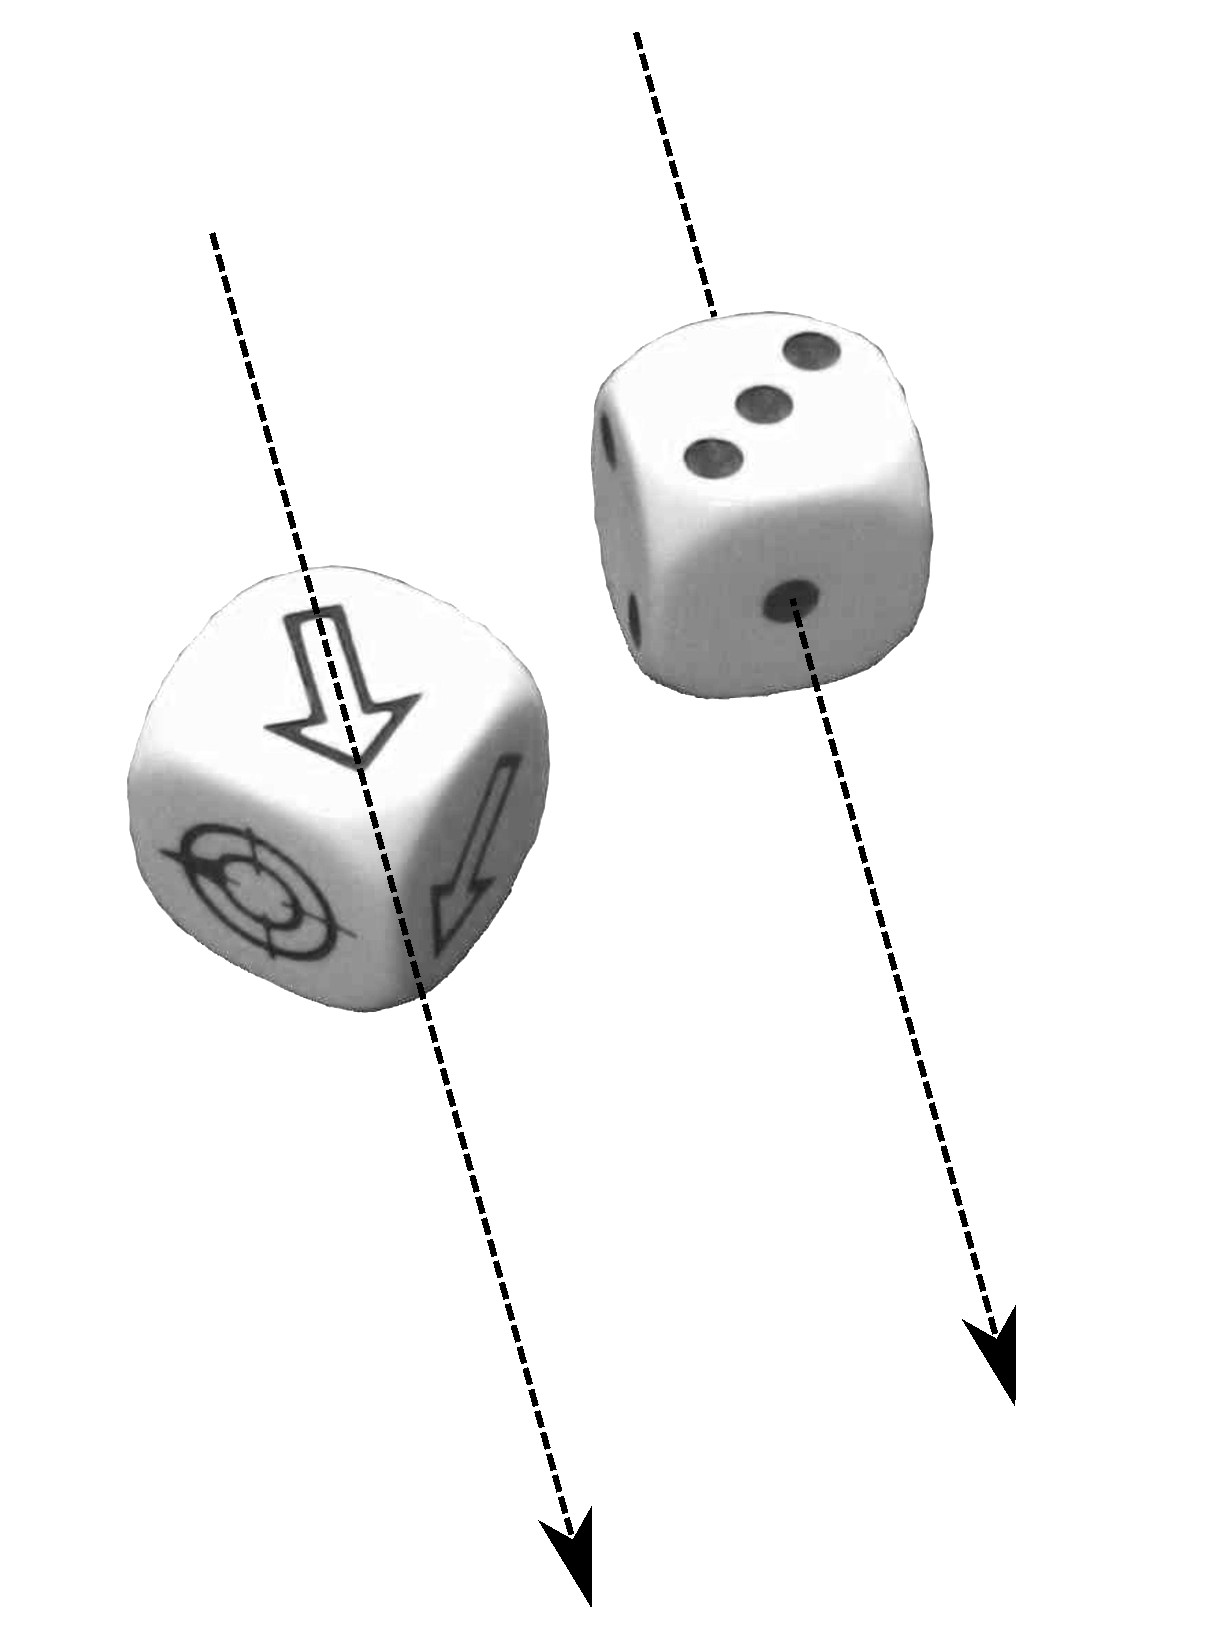
\includegraphics[width=4cm]{de_deviation.png}
\caption{Deux façons équivalentes de représenter un dé de déviation.}
\label{figure/de_deviation}
\end{figure}

\subsection{Déviation}

Quand vous êtes amenés à faire dévier un objet (par exemple \emph{Faites dévier un gabarit de \unit{D6}{\pouce}}), lancez le dé de déviation, et d'autres dés pour la distance si nécessaire. Si un symbole \og Touché ! \fg{} est obtenu, ne bougez pas le gabarit. Si une flèche est obtenue, déplacez le gabarit de la distance indiquée par la description de la règle dans la direction de la flèche. Notez que cela n'est pas la même manipulation que déterminer une direction aléatoire.

\subsection{Direction aléatoire}

Dans certains cas, vous devrez déterminer une direction aléatoire. Lancez le dé de déviation, et si un \og Touché ! \fg{} est obtenu, relancez le dé de déviation jusqu'à obtenir une flèche (exceptionnellement, vous pouvez relancer un dé déjà relancé). Certains dés de déviation ont une petite flèche sur le symbole \og Touché ! \fg{} : pas besoin alors de relancer le dé, utilisez la petite flèche pour la direction.

\section{Gabarits}

Des gabarits sont habituellement utilisés pour déterminer des aires d'effet. Il y a différents types et tailles de gabarits, les plus utilisés étant les gabarits de \unit{3}{\pouce} et \unit{5}{\pouce}. Ce sont des gabarits en forme de disque, dont les diamètres sont \unit{3}{\pouce} et \unit{5}{\pouce}. Il existe également des gabarits moins utilisés comme le gabarit rond de \unit{1}{\pouce} (appelé gabarit de \unit{1}{\pouce}) et le gabarit de ligne (utilisé pour les canons et certains sorts).

Pour définir combien de figurines sont touchées par un gabarit, tenez le gabarit en question au-dessus de la cible pour déterminer quelles figurines ont leur socle directement sous le gabarit. Si n'importe quelle partie du socle d'une figurine, aussi petite soit-elle, est recouverte par le gabarit, la figurine compte comme étant sous le gabarit. Un point du gabarit ne peut être en contact qu'avec un socle au plus. Notez que les socles des figurines sont construits dans une base métrique alors que les tailles des gabarits s'expriment en pouces (\pouce). Cela signifie qu'un gabarit de \unit{3}{\pouce} touche les socles de 5 figurines alignées ayant des socles de \unit{25}{\milli\meter}  (\unit{3}{\pouce} = \unit{7,62}{\centi\meter}).

\subsection{Touches des Gabarits Circulaires}

Les graphiques et le tableau suivant présentent le nombre de figurines qui peuvent être touchées pour chacun des deux Gabarits Circulaires. Voici les dimensions représentées par les couleurs : vert = 20x20 mm, magenta = 25x25 mm, cyan = 40x40 mm et orange = 25x50 mm.

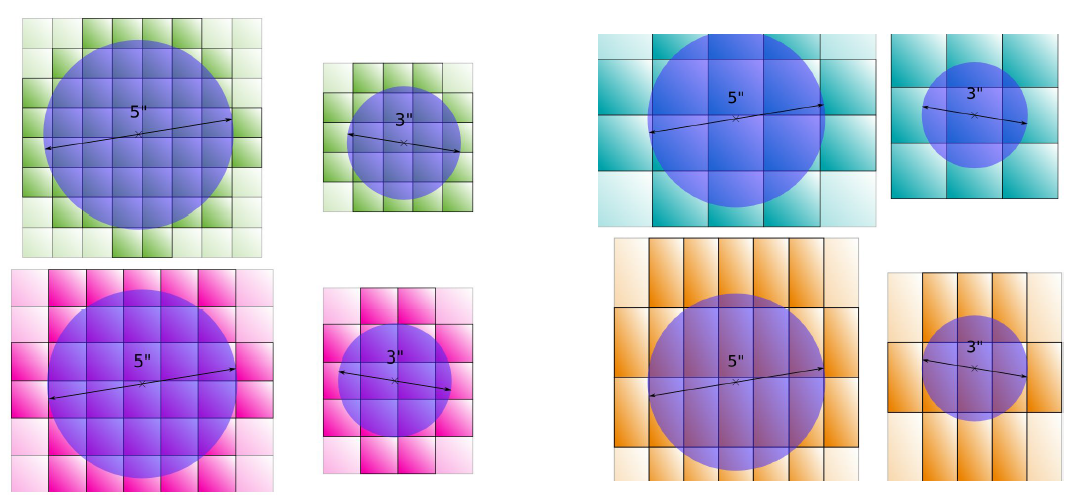
\includegraphics[width=17cm]{gabarits_1.png}

\begin{tabular}{M{2.5cm}|M{2.5cm}M{2.5cm}M{2.5cm}M{2.5cm}}
 & \textbf{Socles 20x20} & \textbf{Socles 25x25} & \textbf{Socles 40x40} & \textbf{Socles 25x50} \\
\hline
\textbf{Gabarit de 3"} & 22 & 16 & 9 & 11 \\
\hline
\textbf{Gabarit de 5"} & 48 & 34 & 16 & 24 \\
\end{tabular}

\subsection{Touches Linéaires}

\begin{figure}[!htbp]
\centering
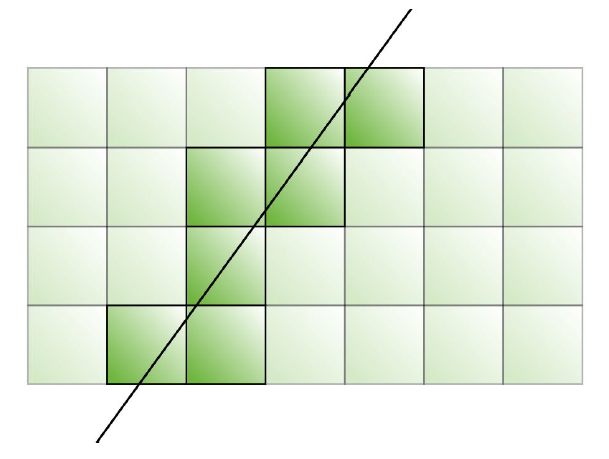
\includegraphics[width=9cm]{gabarits_2.png}
\end{figure}